\section{Introduction}
In order to sucessfully commission the Vera C. Rubin Observatory and begin the Legacy Survey of Space and Time (LSST) we need to be able to perform astrometric and photometric calibrations of individual visits.
Initially, these calibrations will be done within the Rubin Science Pipelines by comparing instrumental measurements of fluxes and positions to those in a reference catalog and deriving photometric zeropoints or astrometric solutions to the World Coordinate System (WCS).
Subsequently, we will use the Forward Global Calibration Method \citep[FGCM;][]{2018AJ....155...41B}, an uber-calibration method, to derive photometric zeropoints for the LSST data and achieve a photometric precision of $\sim$ 1 mmag.
However, during commissioning and early operations our requirements for photometric precision are less rigorous.

The science requirements for photometric repeatability \citep[OSS-REQ-0387;][]{LSE-30} stipulate that the RMS photometric spread of repeated measurements of unresolved sources must be less than 5 mmag (7.5 mmag) for \emph{gri}-band (\emph{uzy}-band) observations.
Additionally, the requirements for the astrometric quality of data are defined in OSS-REQ-0388 such that the median measurement error on the distance between pairs of sources must be less than 10 milli-arcseconds, with an error on the absolute accuracy of positions of less than 50 milliarcseconds in any axis.
To meet these requirements we need a reference catalog with the following features:

\begin{itemize}
    \item The catalog must cover any location we will want to point the telescope.
    For LSST, this includes the full sky with declination < 30 deg, but for completeness we have generated an all-sky catalog.
    \item There must be flux estimates in all bandpasses, \textit{ugrizy} for LSSTCam and \textit{grizy} for LATISS.
    \item The number density of un-saturated high signal-to-noise (S/N) sources must be high enough to calibrate a single LSSTCam CCD.
    This requires there to be at least 10 reference sources per \texttt{NSIDE}=256 healpixel on the sky.
    The size of a detector on the sky is $\sim 0.05\,\mathrm{deg}^2$, equal to the area of an \texttt{NSIDE}=256 healpixel.
    \item High precision measurements of the positions of unresolved sources.
    This is achieved by using \textit{Gaia} Data Release 3 (DR3; \citealt{GaiaCollaboration:2023}) as the basis for the objects in our catalog, with the full high-quality position and proper motion measurements from \textit{Gaia}-DR3 included.
\end{itemize}

Previous catalogs such as ATLAS-REFCAT2 \citep{Tonry:2018} provide all-sky coverage, but are not sufficiently deep to provide the required source density at magnitudes probed by LSST images.
PANSTARRS-1\citep[PS1;][]{Chambers:2016} provides sufficient depth in \emph{grizy}-bands but does not have \emph{u}-band, and its sky coverage is limited to declinations above $\delta = -30$ deg.
Additionally, we would like our reference catalog to provides fluxes in the native LSSTCam (or LATISS) bandpasses to avoid requiring the science pipelines to apply transformations including color terms when processing the data.
Therefore, we have developed \monster, a combination of reference catalogs, containing only stellar sources, similar to ATLAS-REFCAT2 but with the bandpass coverage and depth required to enable LSST.

The code and configuration used to create \monster can be found at \url{https://github.com/lsst-dm/the_monster}\\

\textbf{Note:} We use \emph{source} to describe the bandpass a measurement is currently in and \emph{target} to describe the bandpass we would like to transform a measurement into.

In this document we describe how to access \monster in Section \ref{sec:using}. Section \ref{sec:summary} summarizes the creation of this catalog. In following sections, we discuss in more detail the input datasets (Section \ref{sec:input}), the
conversion of external refcats to the LSST format (Section \ref{sec:conversion}), derivations of the color transformations (Section \ref{sec:colors}), and the stellar locus regression (slr) method used to derive many of the \emph{u}-band fluxes.
Then, in Section \ref{sec:assembly} we present the assembly of \monster including characterizing of version 1 of this catalog.
Finally, we include more detailed descriptions of each of the input catalogs for \monster in Section \ref{sec:details}.

\section{Using \monster}
\label{sec:using}
Version 1 of \monster has been added as a reference catalog to butler repositories at the USDF and the summit.
To access this catalog from the butler use
$$\texttt{datasetType="the\_monster\_20240904"}$$
with the chained collection \texttt{"refcats"} or the run collection \texttt{"refcats/DM-46370/the\_monster\_20240904"}.
The reference catalogs are sharded into \texttt{htm} level 7 trixels; to retrieve a reference catalog, one must thus specify the \texttt{"htm7"} trixel ID in the \texttt{dataId}. Having initialized the butler with, for example:

$$\texttt{from lsst.daf.butler import Butler}$$
$$\texttt{butler = Butler("embargo", collections="refcats")}$$

one can then retrieve a reference catalog for a given htm id (in this case, \texttt{"htm7=203118"}) via the following:

$$\texttt{refcat = butler.get("the\_monster\_20240904", dataId=\{"htm7":203118\})}$$

ADD MORE DETAIL HERE ABOUT WHAT'S IN THE CATALOGS.

For each photometric system and bandpass in \monster there are three columns: 
\begin{itemize}
    \item \texttt{monster\_\{system\}\_\{band\}\_flux}: estimated flux in band of system 
    \item \texttt{monster\_\{system\}\_\{band\}\_fluxErr}: estimated fluxErr in band of system 
    \item \texttt{monster\_\{system\}\_\{band\}\_source\_flag}: source of observation estimate was derived from.  
\end{itemize}

The systems and bands included are:
\begin{itemize}
    \item DES: grizy
    \item SDSS: u
    \item LATISS: grizy
    \item SynthLSST: ugrizy.
\end{itemize}

The flat files for \monster in fits format can be accessed at the USDF at the location
$$\texttt{path=/sdf/group/rubin/shared/refcats/the\_monster\_20240904/}$$


\section{Summary of creation of \monster}
\label{sec:summary}
The creation of the \monster can divided into two components, the \textit{grizy}-bands and the \textit{u}-band. 


\subsection{\textit{grizy-bands}}
\begin{enumerate}
    \item For each input reference catalog, we retrieve a version containing only high-quality stellar sources. This process is generally described in Section \ref{sec:input} and details for each external input refcat are discussed in Section \ref{sec:details}
    \item Subsequently, all input catalogs are converted into the LSST refcat format (htm7), see Section \ref{sec:conversion}.
    \item Our reference catalog, \monster, uses DES bandpasses internally for \textit{grizy}-bands. So, the next step is to convert all measured fluxes to the DES system by derving color transformations. 
    This is done by fitting a cubic spline to the ratio of source flux and target flux as a function of color for a high quality subset of the data over a restricted color range.
    \item With the external reference catalogs in hand, as well as colorterms for each measurement, we can create versions of each source-refcat (e.g PS1) that have been matched to \textit{Gaia\_DR3} sources, further selected to only include isolated sources (no neighbors within 1"), and transformed to the DES bandpass.
    \item Finally, we assemble \monster by reading in each transformed htm shard and adding measurements for each \textit{Gaia\_DR3} (a rank order of preference is used when multiple refcats have measurements of the same source) to the\_monster catalog. 
    We add flux measurements for the DES-bandpasses as well as any target bandpasses for the\_monster catalog. In version one of the\_monster, \textit{the\_monster\_20240904}, LATISS fluxes and synthLSST fluxes are included as well.
\end{enumerate}

\subsection{u-band}
For the \textit{u}-band, the creation process is similar with a few notable exceptions:
\begin{itemize}
    \item The internal refcat system is SDSS \textit{u}-band instead of the DES-bandpasses.
    \item The sources used to derive measurements are in the same manner as the rest of the \monster are SDSS \textit{u}-band measurements and $\mathrm{GaiaXP_{SDSSu}}$ photometry. 
    Unfortunately, the density of sources with SDSS \textit{u}-band or $\mathrm{GaiaXP_{SDSSu}}$ is not high enough over the full LSST footprint. 
    \item 
    Therefore, we additionally use a stellar locus regression-based (SLR) method to estimate the \textit{u}-band flux for an additional set of stars. 
    This SLR method uses DES \textit{g}-band fluxes and \textit{g-r} colors to estimate the SDSS \textit{u}-band measurements and is described in Section \ref{sec:slr}
\end{itemize}

\section{Input Data}
\label{sec:input}
Here we describe the input catalogs used for the creation of \monster. 
%For each catalog, we include the origin, any cuts applied, and summary plots of the spatial distributions. 
The photometric catalogs used in this process for the \emph{grizy}-bands are (in order of priority):
\begin{enumerate}
    \item DES Y6 Calibration Stars (\ref{sec:des})
    \item Gaia XP Synthetic Magnitudes (\ref{sec:gaiaxp})
    \item PS1 (\ref{sec:ps1})
    \item SkyMapper (\ref{sec:skymapper})
    \item VST (\ref{sec:vst})
\end{enumerate}

For \textit{u}-band we use:
\begin{itemize}
    \item SDSS Standard Stars (\ref{sec:sdss})
    \item Gaia XP Synthetic Magnitudes (\ref{sec:gaiaxp})
    \item Stellar Locus Regression-based magnitudes (SLR) (\ref{sec:slr})
\end{itemize}

\section{Catalog conversion}
\label{sec:conversion}
To convert the catalogs into LSST format, we follow the instructions on \href{https://pipelines.lsst.io/modules/lsst.meas.algorithms/creating-a-reference-catalog.html}{pipelines.lsst.io} on how to generate an LSST reference catalog using the \href{https://pipelines.lsst.io/modules/lsst.meas.algorithms/tasks/lsst.meas.algorithms.ConvertReferenceCatalogTask.html#lsst-task-lsst-meas-algorithms-convertreferencecatalog-convertreferencecatalogtask}{ConvertReferenceCatalogTask}. Each refcat requires its own configurations, which can be found in the \href{https://github.com/lsst-dm/the_monster/tree/main/configs}{\texttt{/configs/} folder of the\_monster github repo}.
This conversion process shards the catalog into htm=7 trixels and creates a set of standard columns that include ra/dec coordinates as well as fluxes and errors in units of nJy.

\section{Color Transformations}
\label{sec:colors}
The creation of \monster v1 required a number of different types of color transformations. 
In this section we describe the derviation of these color transformations and show a few examples. 
We include diagnostic plots for all color transformations used in \monster in appendix \ref{app:colorplots}
Initially, all of the inuput catalogs flux measurements must be transformed into the internal bandpasses of \monster (DES for \emph{grizy}-band SDSS for \emph{u}-band); sections \ref{sec:todes} and \ref{sec:tosdss} show examples of this process. 
Subsequently, during the assembly of \monster, the internal bandpasses must be transformed into the target bandpasses for \monster. 
This is done using estimated transmissions for LSST and emprically for LATISS. 

% want a table with inital cat, target cat, number of nodes, color range, fit flux offset, source flag

\subsection{Fitting color transformations}
To derive color transformations we perform a cubic-spline based fit to derive a relation between a color mesurement the initial photometric bandpass and the ratio of fluxes between the inital and target bandpasses.
For example, the transformation from GaiaXP's estimate of DES g-band (initial bandpass) to DES g-band (target bandpass) is shown as a red line in figure \ref{fig:color-xp-g}. 
These transformation are derived using the \href{https://github.com/lsst-dm/the_monster/blob/main/python/lsst/the/monster/measure_colorterms.py}{SplineMeasurer} class from \monster. 

This fit is done by taking a spatial region where the source and target refcats overlap. 
Over this region we 1) read in the source refcat, target refcat, and \emph{Gaia}DR3, 2) we spatially match the source and target refcats to \emph{Gaia}DR3. 3) in the source catalog we apply a single band, \textit{i}-band by default, selection to obtain a sample of high-quality stellar-sources.  

With a matched catalog containing flux measurements in both systems in hand, we compute g-i (i-z) colors for all objects in gri-bands (zy-bands). 
These colors are used to select a subest sources that we expect to be well behaved, the color ranges for each transfomation are listed in table ..... .
Next, we fit a cubic spline to the data using equally spaced nodes over the color range.
If necessary the color terms include a flux offset to bring the two systems into agreement. 
In a few cases, such as PS1 to DES we find a magnitude-dependent offset that has been fit as well.

\subsection{To DES Bandpasses}
\label{sec:todes}
%Here we show an example of 
\begin{figure}
    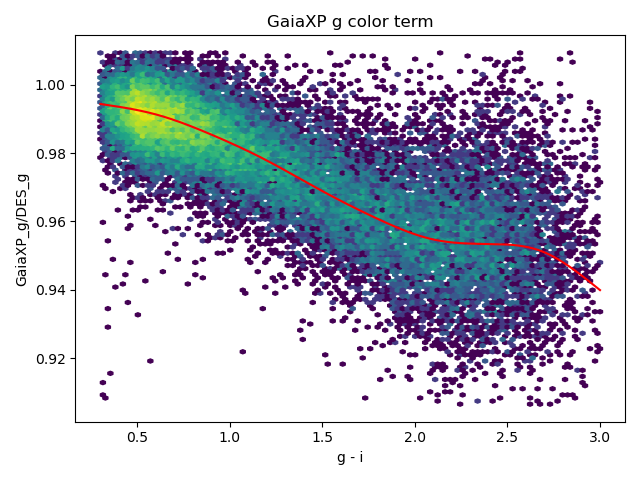
\includegraphics[width=0.49\linewidth]{./figures/color_terms/GaiaXP_to_DES_band_g_color_term.png}
    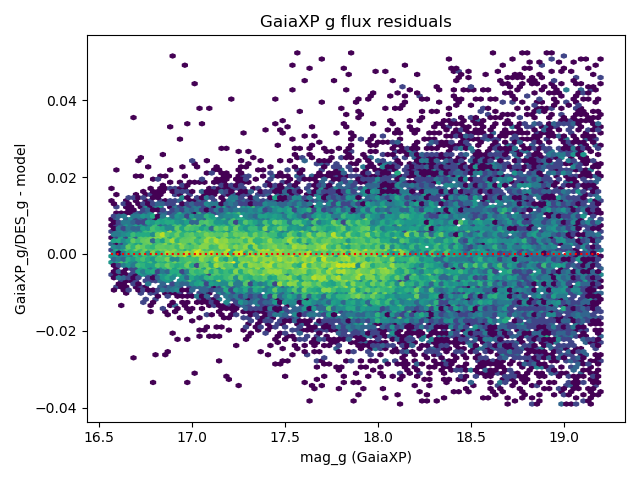
\includegraphics[width=0.49\linewidth]{./figures/color_terms/GaiaXP_to_DES_band_g_flux_residuals.png}
    \caption{Left: The ratio of fluxes between GaiaXP synthetic photometry and DES for the \textit{g}-band as a function of \textit{g-i} color. The red line shows the cubic spline that defines our color transformation.
    Right: Residuals between GaiaXP synthetic photometry transformed to DES and DES as a function of magnitude.}
    \label{fig:color-xp-g}
\end{figure}
\subsection{To SDSS \textit{u}-band}
\label{sec:tosdss}
Need to go find/make these figures. 
% \begin{figure}
%     \includegraphics[width=0.49\linewidth]{./figures/color_terms/GaiaXP_to_SDSS_band_u_color_term.png}
%     \includegraphics[width=0.49\linewidth]{./figures/color_terms/GaiaXP_to_SDSS_band_u_color_term.png}
%     \caption{Left: The ratio of fluxes between GaiaXP synthetic photometry and DES for the \textit{g}-band as a function of \textit{g-i} color. The red line shows the cubic spline that defines our color transformation.
%     Right: Residuals between GaiaXP synthetic photometry transformed to DES and DES as a function of magnitude.}
%     \label{fig:color-xp-u}
% \end{figure}
\subsection{To Synthetic LSST Bandpasses}
\begin{itemize}
    \item FGCM star templates cite rykoff fgcm? 
    \item baseline v1.9 lsst transmissions \url{https://raw.githubusercontent.com/lsst/throughputs/main/baseline/total_{filter_}.dat}
    \item des passbands \url{https://noirlab.edu/science/sites/default/files/media/archives/documents/scidoc1884.txt}
    \item estimated color terms!
\end{itemize}
\subsection{To LATISS Bandpasses}
\begin{itemize}
    \item fgcm stars from coadd run. What collection when was the data taken? 
\end{itemize}
\begin{figure}
    \includegraphics[width=0.49\linewidth]{./figures/color_terms/DECam_monster_to_LATISS_band_g_color_term.png}
    \includegraphics[width=0.49\linewidth]{./figures/color_terms/DECam_monster_to_LATISS_band_g_flux_residuals.png}
    \caption{Left: The ratio of fluxes between GaiaXP synthetic photometry and DES for the \textit{g}-band as a function of \textit{g-i} color. The red line shows the cubic spline that defines our color transformation.
    Right: Residuals between GaiaXP synthetic photometry transformed to DES and DES as a function of magnitude.}
    \label{fig:color-des-latiss-g}
\end{figure}

\section{Stellar Locus Regression for the \textit{u}-band}
\label{sec:slr}

\begin{itemize}
    \item find some citations for SLR
    \item magic 
\end{itemize}
The SLR method we employed uses 
%- for a set of stars with SDSS-u and DES g/r measurements we derive colorterms?

\section{Assembly of the\_monster v1}
\label{sec:assembly}



% g
\begin{figure}
    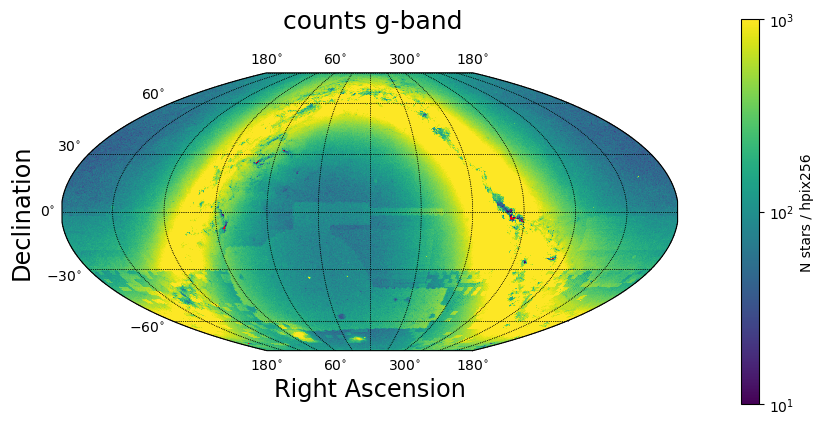
\includegraphics[width=0.48\linewidth]{./figures/source_density_maps/g-band_counts_full.png}
    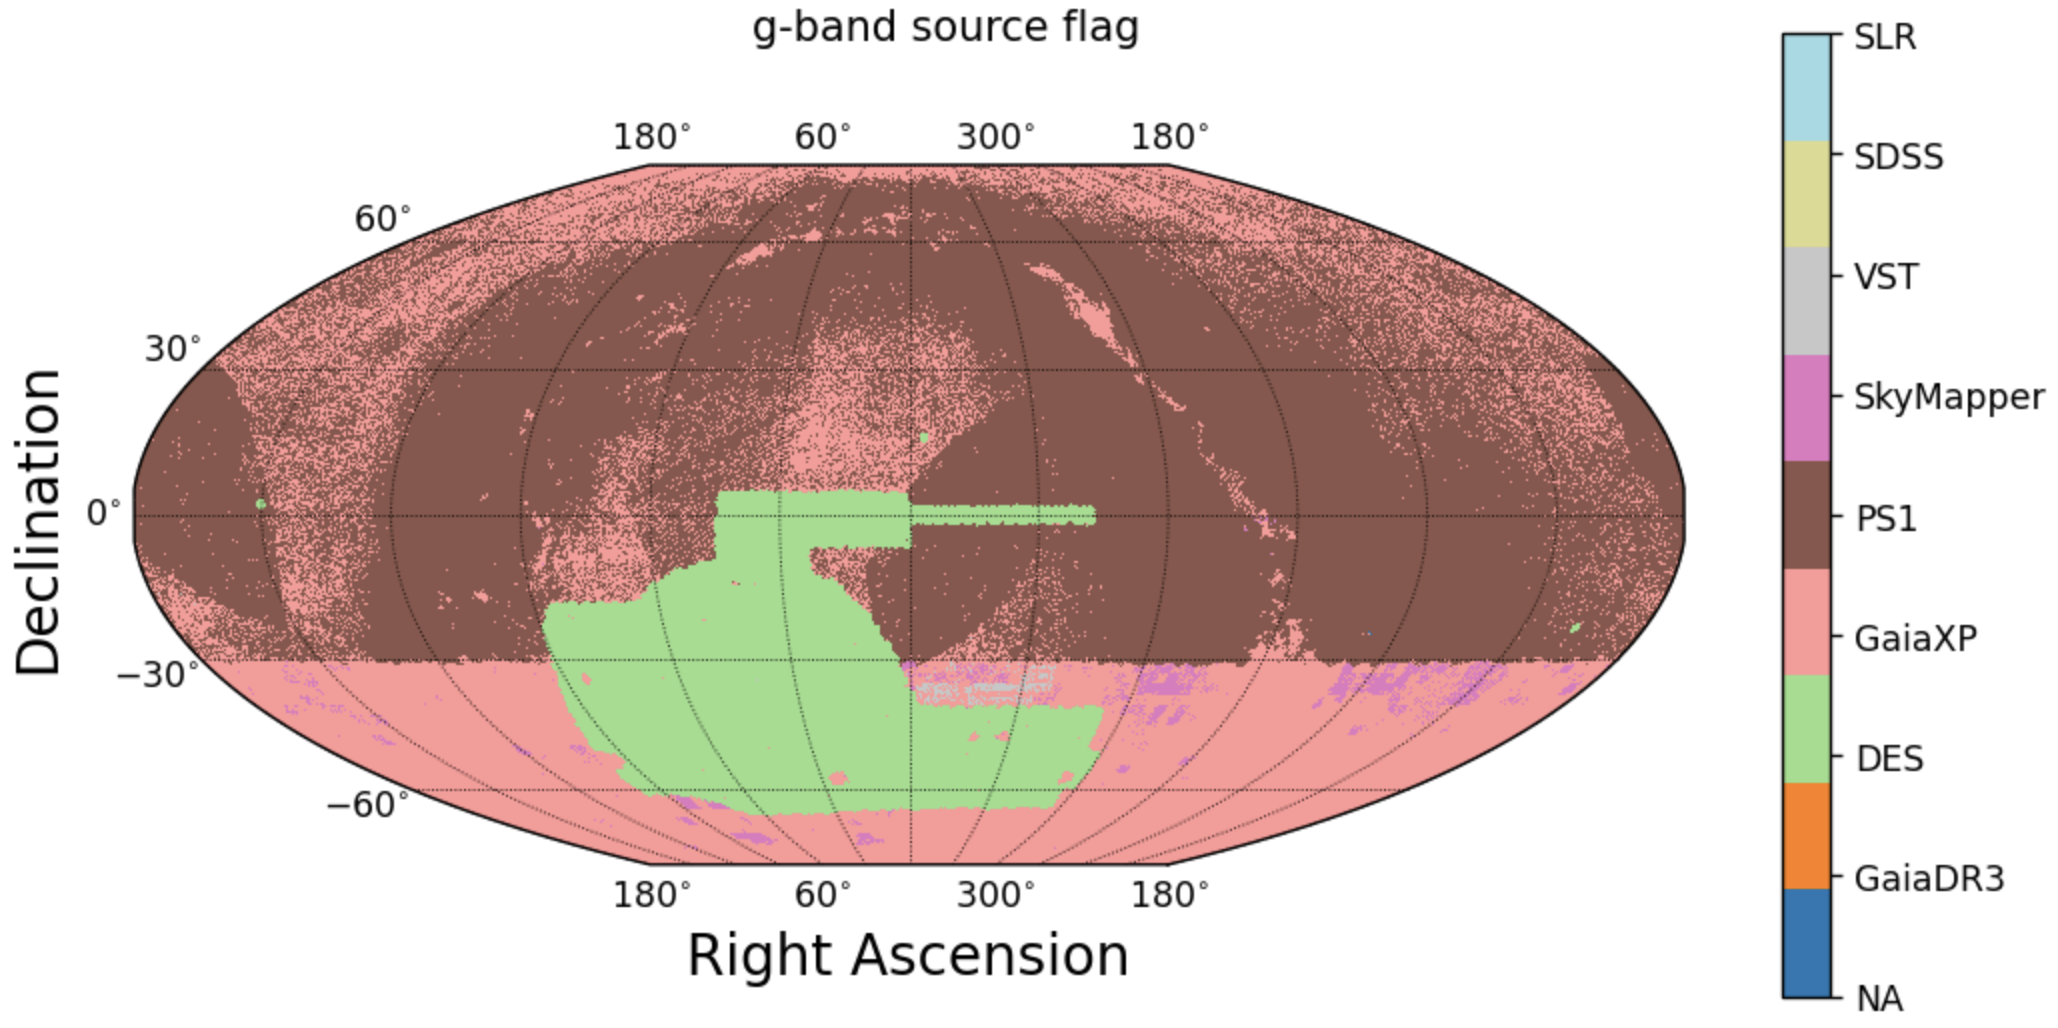
\includegraphics[width=0.48\linewidth]{./figures/source_survey_maps/g-band_source.png}
    \caption{Left: Map showing the number of sources with a \textit{g}-band measurement per \texttt{nside}=256 healpixel.
    Right: Map showing the median source of objects at each point in the sky for the \textit{g} band.}
    \label{fig:monster-g}
\end{figure}
% r 
\begin{figure}
    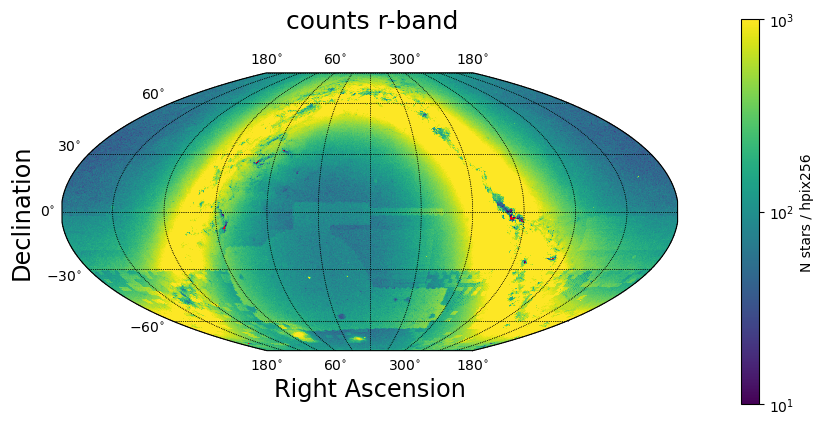
\includegraphics[width=0.48\linewidth]{./figures/source_density_maps/r-band_counts_full.png}
    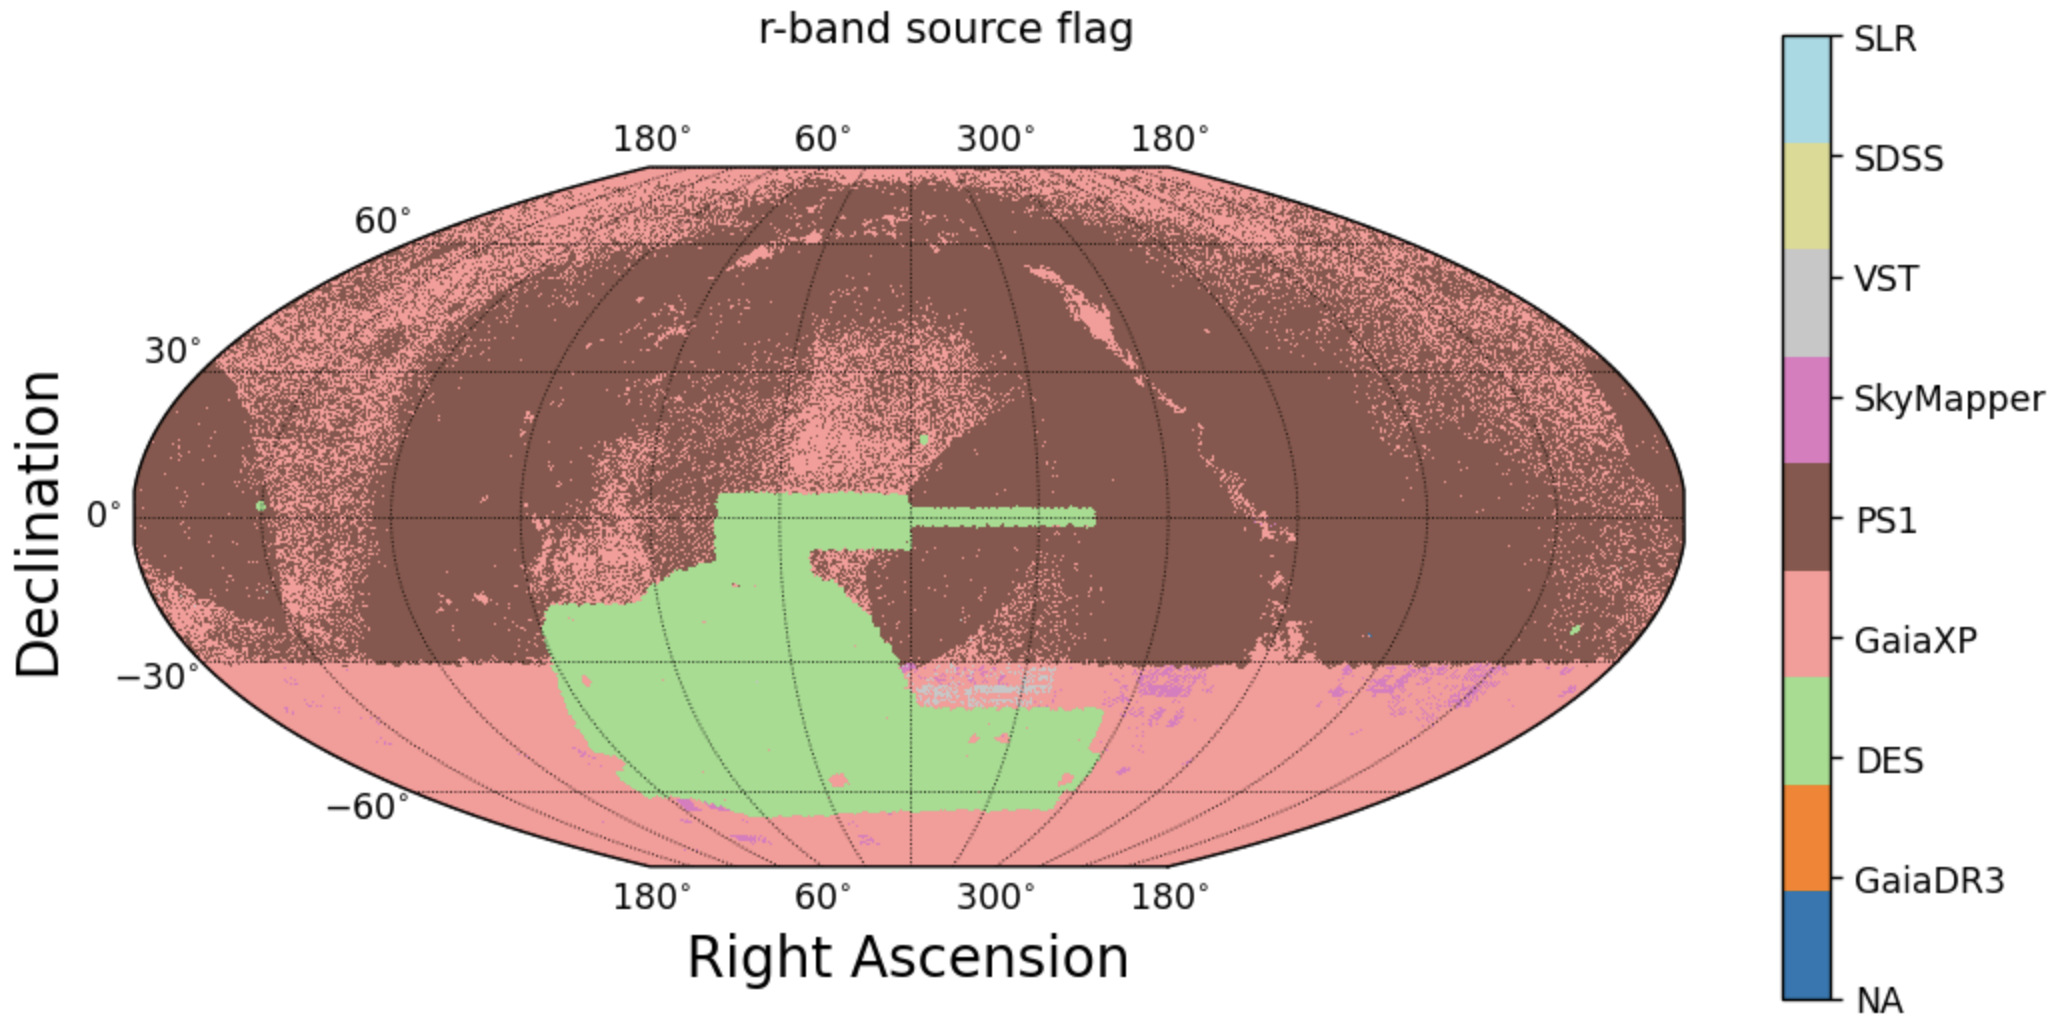
\includegraphics[width=0.48\linewidth]{./figures/source_survey_maps/r-band_source.png}
    \caption{Left: Map showing the number of sources with a \textit{r}-band measurement per \texttt{nside}=256 healpixel.
    Right: Map showing the median source of objects at each point in the sky for the \textit{r} band.}
    \label{fig:monster-r}
\end{figure}
% i
\begin{figure}
    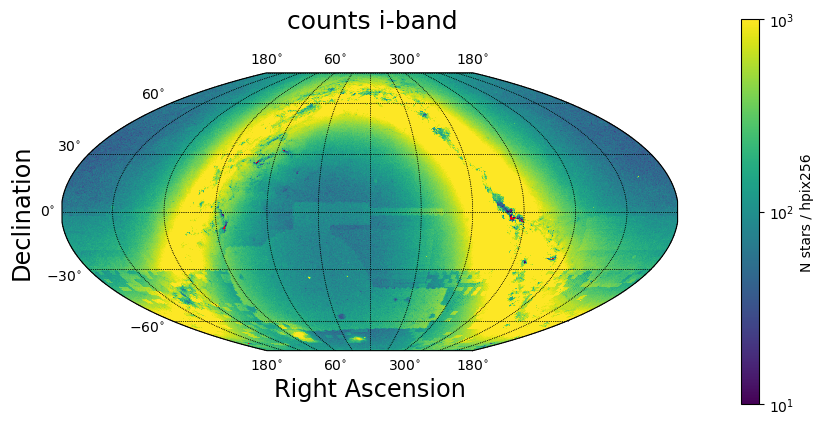
\includegraphics[width=0.48\linewidth]{./figures/source_density_maps/i-band_counts_full.png}
    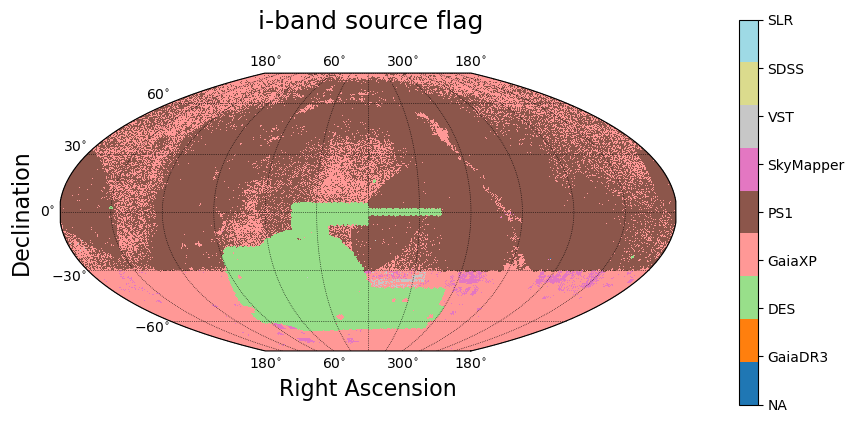
\includegraphics[width=0.48\linewidth]{./figures/source_survey_maps/i-band_source.png}
    \caption{Left: Map showing the number of sources with a \textit{i}-band measurement per \texttt{nside}=256 healpixel.
    Right: Map showing the median source of objects at each point in the sky for the \textit{i} band.}
    \label{fig:monster-i}
\end{figure}
% z
\begin{figure}  
    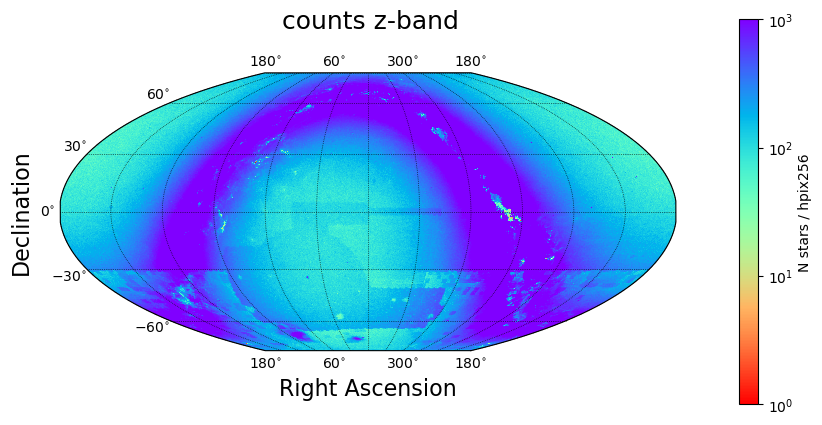
\includegraphics[width=0.48\linewidth]{./figures/source_density_maps/z-band_counts_full.png}
    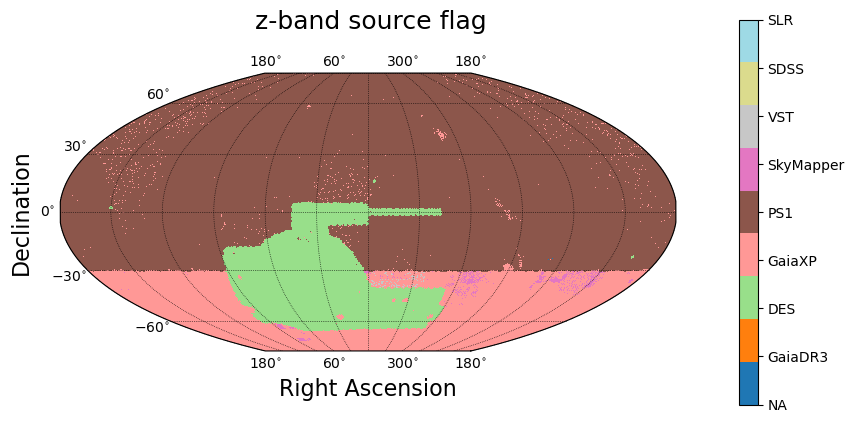
\includegraphics[width=0.48\linewidth]{./figures/source_survey_maps/z-band_source.png}
    \caption{Left: Map showing the number of sources with a \textit{z}-band measurement per \texttt{nside}=256 healpixel.
    Right: Map showing the median source of objects at each point in the sky for the \textit{z} band.}
    \label{fig:monster-z}
\end{figure}
% y
\begin{figure}
    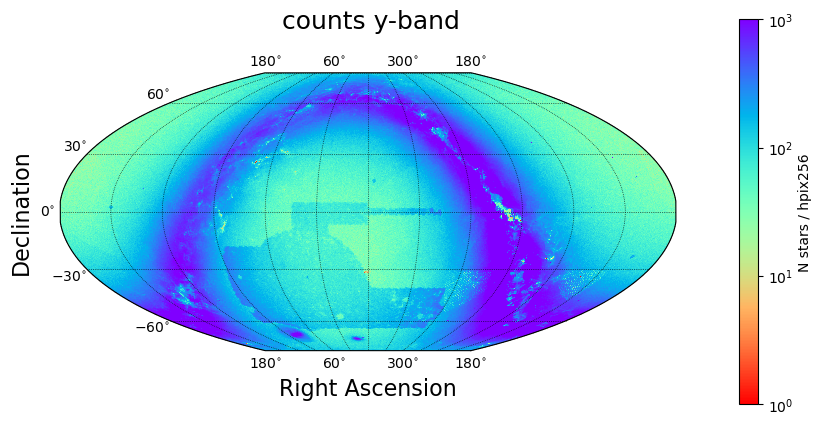
\includegraphics[width=0.48\linewidth]{./figures/source_density_maps/y-band_counts_full.png}
    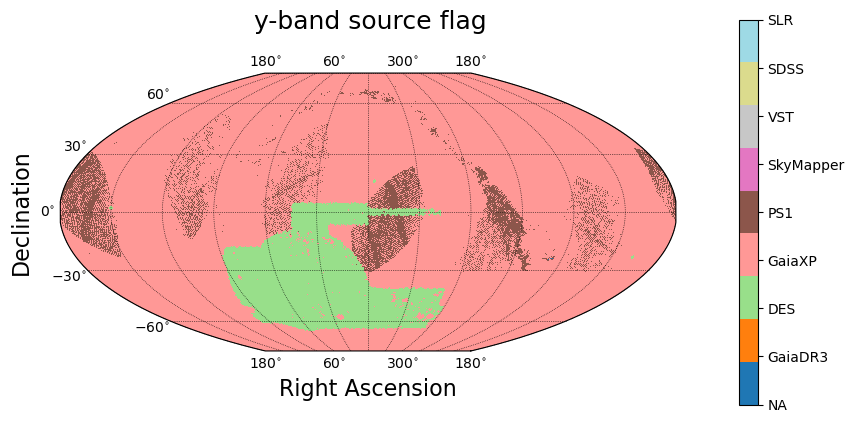
\includegraphics[width=0.48\linewidth]{./figures/source_survey_maps/y-band_source.png}
    \caption{Left: Map showing the number of sources with a \textit{y}-band measurement per \texttt{nside}=256 healpixel.
    Right: Map showing the median source of objects at each point in the sky for the \textit{y} band.}
    \label{fig:monster-y}
\end{figure}

\section{Detailed Descriptions}
\label{sec:details}
In the following subsections, we describe the external photometric catalogs used in the creation of the\_monster.

\subsection{Dark Energy Survey (DES) Y6 Calibration Stars}
\label{sec:des}
Data is described in \href{https://arxiv.org/abs/2305.01695}{Rykoff et al 2023}.
Briefly, this is a catalog of calibrated reference stars generated by the Forward Calibration Method (FGCM) pipeline (arXiv:1706.01542) as part of the FGCM photometric calibration of the full Dark Energy Survey (DES) 6-Year data set (Y6). This catalog provides DES \textit{grizY} magnitudes for 17 million stars with \textit{i}-band magnitudes mostly in the range 16 < \textit{i} < 21, spread over the full DES footprint covering 5000 square degrees over the Southern Galactic Cap at galactic latitudes \textit{b} < -20 degrees (plus a few outlying fields disconnected from the main survey footprint). 
These stars are calibrated to a uniformity of better than 1.8 milli-mag (0.18\%) RMS over the survey area. 
The absolute calibration of the catalog is computed with reference to the STISNIC.007 spectrum of the Hubble Space Telescope CalSpec standard star C26202; including systematic errors, the absolute flux system is known at the approximately 1\% level. 
These stars provide a useful reference catalog for calibrating \textit{grizY}-band or \textit{grizY}-like band photometry in the Southern Hemisphere, particularly for observations within the DES footprint.

The data was retrieved from \url{https://data.darkenergysurvey.org/public_calib/DES_6yr_CalibStarCat/Y6A1_FGCM_V3_3_1_PSF_ALL_STARS.fits}.

More information can be found at \url{https://des.ncsa.illinois.edu/releases/other}

% \subsubsection{Color transformations}
% The DES bandpasses act as the internal bandpasses for \monster and 

\subsection{Gaia XP Synthetic Magnitudes}
\label{sec:gaiaxp}
As inputs to \monster we use synthetic photometry derived from the Gaia DR3 XP spectra \citep{GaiaCollaboration:2023}. 
The synthetic photometry is dervied from low-resolution spectrophotometry of ~220 million sources in the wavelength range 330nm - 1050nm. 
This is done using the \href{https://github.com/gaia-dpci/GaiaXPy/cd}{GaiaXPy} package. 
GaiaXPy uses measured DECam-grizy and SDSS-u transmission curves to generate synthetic photometry in each bandpass. 


\subsection{PanSTARRS1 (PS1)}
\label{sec:ps1}

We use data from the Pan-STARRS1 3pi survey, released to the Pan-STARRS1 Science Consortium.
In particular, the refcat is constructed from the "3pi.pv3.20160422" DVO catalog of Processing Version 3.
The catalog contains $2.9 \times 10^9$ point sources at Dec > -30 deg to i $\sim$ 22.5 mag,

For more information see \href{http://panstarrs.stsci.edu} and \citet{Chambers:2016}.

\subsection{SkyMapper}
\label{sec:skymapper}
For \monster we use DR2 of the SkyMapper catalog \citep{Onken:2019} downloaded from \href{https://skymapper.anu.edu.au/_data/DR2/}. 
This catalog contains ugriz photometry of over $500 \times 10^6$ objects with \textit{r}-band magnitudes ranging from 10-21. 

\subsection{VST}
\label{sec:vst}

VST ATLAS DR4 downloaded from ESO archive.

Documentation can be found at: \url{http://www.eso.org/rm/api/v1/public/releaseDescriptions/90}

Skim to healpixels was done with the following criteria:
\begin{verbatim}
sel = (dat["MERGEDCLASS"] == -1)  # stars
sel &= (dat["PRIORSEC"] == 0)     # unique source 
sel &= (dat["PRIMARY_SOURCE"] == 1) # primary source 
sel &= (dat["UERRBITS"] < 0)      # no u-band processing flags
\end{verbatim}

\subsection{GAIA DR3 - The Astrometric Reference}
\label{sec:gaiadr3}
Original data: \url{https://www.cosmos.esa.int/web/gaia/dr3}

The full Gaia DR3 catalog in indexed HTM format. 
This is the first LSST refcat to contain the full coordinate covariance.

Magnitude range: $\sim$3 - 21 (G magnitude)

\subsection{SDSS}
\label{sec:sdss}


% \section*{Methods}

% \subsection*{grizy-bands}
% \begin{enumerate}
%     \item Cross-match each catalog to Gaia DR3 (after some isolation cuts).
%     \item Use the Gaia/DES cross-match stars as the overall cross-calibration reference.
%     \item For each catalog, compute an empirical correction to go from Catalog X to DES. This uses the cross-coverage. The empirical correction will be some sort of spline fit (TBD) to apply to stars across a broad range of colors. We will also allow for a "background offset" term (to account for offsets as a function of flux due to background issues).
%     \item Apply the empirical correction to convert Catalog X to DES bands for the full catalog.
%     \item Convert from DES to LSSTCam (sim for now) using a stellar template library. When we have real data (throughputs, stars, both), we can update this conversion all at once.
%     \item Choose a catalog rank-ordering (e.g., DES, Gaia XP, PS1, SkyMapper, etc.).
%     \item For each star with band X, choose the top-ranked catalog with a measurement in that band.
% \end{enumerate}

% \subsection*{u-band}
% \begin{enumerate}
%     \item XP (SDSS) \textit{g-r/u} to SDSS \textit{u} correction, with a northern training region at high latitude.
%     \item DES \textit{g-r} to corrected XP corrected SDSS \textit{u} over DES training region at high latitude.
%     \item Over the full Monster footprint, estimate SDSS SLR \textit{u} for all stars where we have a \textit{g-r} color estimate (DES equivalent).
%     \item Over the full Monster footprint, at low resolution, estimate the offset between the XP corrected SDSS \textit{u} and the SLR \textit{u}.
%     \item Use bilinear interpolation to correct the SLR \textit{u} to the XP \textit{u} so everything will be well matched.
% \end{enumerate}


